\documentclass[paper=letter,fontsize=11pt]{scrartcl} % KOMA-article class
							
\usepackage[english]{babel}
\usepackage[utf8x]{inputenc}
\usepackage[protrusion=true,expansion=true]{microtype}
\usepackage{amsmath,amsfonts,amsthm}     % Math packages
\usepackage{graphicx}                    % Enable pdflatex
\usepackage[svgnames]{xcolor}            % Colors by their 'svgnames'
\usepackage{geometry}
	%\textheight=700px                    % Saving trees ;-)
%\usepackage{url}
\usepackage[colorlinks=true,
linkcolor=blue,
urlcolor=blue]{hyperref}
\usepackage{float}
\usepackage{etaremune}
\usepackage{wrapfig}

\usepackage{attachfile}

\frenchspacing              % Better looking spacings after periods
%\pagestyle{empty}           % No pagenumbers/headers/footers
\usepackage{lastpage}
\usepackage{fancyhdr}
\pagestyle{fancy} 
\cfoot{\thepage\ of \pageref{LastPage}}
%\addtolength{\voffset}{-40pt}
%\addtolength{\textheight}{20pt}

\setlength\topmargin{0pt}
\addtolength\topmargin{-\headheight}
\addtolength\topmargin{-\headsep}
\setlength\oddsidemargin{0pt}
\setlength\textwidth{\paperwidth}
\addtolength\textwidth{-2in}
\setlength\textheight{\paperheight}
%\addtolength\textheight{-3in}
\addtolength\textheight{-2in}
\usepackage{layout}

%%% Custom sectioning}{sectsty package)
%%% ------------------------------------------------------------
\usepackage{sectsty}

\sectionfont{%			            % Change font of \section command
	\usefont{OT1}{phv}{b}{n}%		% bch-b-n: CharterBT-Bold font
	\sectionrule{0pt}{0pt}{-5pt}{3pt}}

%%% Macros
%%% ------------------------------------------------------------
\newlength{\spacebox}
\settowidth{\spacebox}{8888888888}			% Box to align text
\newcommand{\sepspace}{\vspace*{1em}}		% Vertical space macro

\newcommand{\MyName}[1]{ % Name
		\Huge \usefont{OT1}{phv}{b}{n} \hfill #1
		\par \normalsize \normalfont}
		
\newcommand{\MySlogan}[1]{ % Slogan}{optional)
		\large \usefont{OT1}{phv}{m}{n}\hfill \textit{#1}
		\par \normalsize \normalfont}

\newcommand{\NewPart}[2]{\section*{\uppercase{#1} #2}}

\newcommand{\PersonalEntry}[2]{
		\noindent\hangindent=2em\hangafter=0 % Indentation
		\parbox{\spacebox}{        % Box to align text
		\textit{#1}}		       % Entry name}{birth, address, etc.)
		\hspace{1.5em} #2 \par}    % Entry value

\newcommand{\SkillsEntry}[2]{      % Same as \PersonalEntry
		\noindent\hangindent=2em\hangafter=0 % Indentation
		\parbox{\spacebox}{        % Box to align text
		\textit{#1}}			   % Entry name}{birth, address, etc.)
		\hspace{1.5em} #2 \par}    % Entry value	
		
\newcommand{\EducationEntry}[4]{
		\noindent \textbf{#1} \hfill      % Study
		\colorbox{White}{%
			\parbox{6em}{%
			\hfill\color{Black}#2}} \par  % Duration
		\noindent \textit{#3} \par        % School
		\noindent\hangindent=2em\hangafter=0 \small #4 % Description
		\normalsize \par}

\newcommand{\WorkEntry}[4]{				  % Same as \EducationEntry
		\noindent \textbf{#1} \hfill      % Jobname
		\colorbox{White}{\color{White}#2} \par  % Duration
		\noindent \textit{#3} \par              % Company
		\noindent\hangindent=2em\hangafter=0 \small #4 % Description
		\normalsize \par}

\newcommand{\PaperEntry}[7]{
		\noindent #1, ``\href{#7}{#2}", \textit{#3} \textbf{#4}, #5 (#6).}

\newcommand{\ArxivEntry}[3]{
		\noindent #1, ``\href{http://arxiv.org/abs/#3}{#2}", \textit{{cond-mat/}#3}.}
        
\newcommand{\BookEntry}[4]{
		\noindent #1, ``\href{#3}{#4}", \textit{#3}.}
        
\newcommand{\FundingEntry}[5]{
        \noindent #1, ``#2", \$#3 (#4, #5).}

\newcommand{\TalkEntry}[4]{
		\noindent #1, #2, #3 #4}

\newcommand{\ThesisEntry}[5]{
		\noindent #1 -- #2 #3 ``#4" \textit{#5}}

\newcommand{\CourseEntry}[3]{
		\noindent \item{#1: \textbf{#2} \\ #3}}

%%% Begin Document
%%% ------------------------------------------------------------
\begin{document}

%\layout

% you can upload a photo and include it here...
\begin{wrapfigure}{l}{0.5\textwidth}
	\vspace*{-2em}
		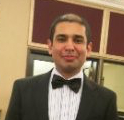
\includegraphics[width=0.18\textwidth]{Fahad.jpg}
\end{wrapfigure}

\MyName{Syed F. Naeem}
\MySlogan{Curriculum Vit\ae\ (\today)}

\sepspace

%%% Personal details
%%% ------------------------------------------------------------
\NewPart{}{}

\PersonalEntry{Address}{C/o Mia Strömsholm, Barrskogsgatan 5, Göteborg, Sweden}
\PersonalEntry{Phone}{+46(0) 73-652-9380}
\PersonalEntry{Mail}{\href{mailto:syed@nephy.chalmers.se, sfnaeem@gmail.com}{syed@nephy.chalmers.se, sfnaeem@gmail.com}}
\PersonalEntry{WWW}{\href{http://nephy.chalmers.se/safeguards/index.html}{http://nephy.chalmers.se/safeguards/index.html}}


%%% Work experience
%%% ------------------------------------------------------------
\NewPart{Appointments}{}


\EducationEntry{Senior Researcher}{2015-$\qquad$}{Department of Applied Physics, Chalmers University of Technology, Göteborg, Sweden}{\begin{itemize}
\item{Nuclear Safeguards Research: Develop methods and techniques for radiation detection and measurements using organic-liquid and NaI(Tl) scintillators, and validate Monte Carlo simulations against measurements taken at the Joint Research Center facility in Ispra, Italy}
\item{Radiological Safety: Measurements taken in the proton accelerator facility to determine the origin of high neutron dose rates (22 \(\mu\)Sv/h) at the Institut des Microtechnologies Appliquées in La Chaux-de-Fonds, Switzerland}
\item{Data analysis software development to read and process the fission chambers binary data obtained in the GANDDALF (Guinevere ANalog Digital Data Acquisition at moL Facility) data format}
\item{Work in collaboration with the space sciences research group at Chalmers University of Technology to irradiate Si wafers used in Balometers}
\item{\textit{Teaching:} Radiation measurements laboratory}\end{itemize}}
\sepspace

\EducationEntry{Postdoctoral Research Fellow}{2011-2014}{Department of Nuclear Engineering \& Radiological Sciences, University of Michigan, Ann Arbor, Michigan, United States}{\begin{itemize}
\item{Experimental and analytical/Monte Carlo research with the Detection for Nuclear Nonproliferation Group}
\item{Equipment: CAEN V1720 12-bit 250 MS/s waveform digitizer, EJ-309 and BC-501A organic-liquid and NaI scintillators used in measurements; Monte Carlo simulations done in the high-performance computing cluster}
\item{Research Mentor}{\textit{Undergraduate Research Opportunity Program}}
\subitem{\underline{Students:} Julia Milton (2012), Brandon LaFleur (2013), Matthew O'Callaghan (2013),}
\subitem{and Yashwanth Lagisetty (2014)}
\item{\textit{Teaching:} Monte Carlo simulations module and relevant laboratory experiments in NERS 535 (course code): “Detection Techniques for Nuclear Nonproliferation” (3 credits)}

\end{itemize}}
\sepspace

\EducationEntry{Graduate Research Assistant}{2005-2010}{Department of Physics and Idaho Accelerator Center, Idaho State University, Pocatello, Idaho, United States}{\begin{itemize}
\item \underline{PhD project:} Utilization of tunable and quasi-monochromatic Laser-Compton Scattered x-rays for nuclear processing streams identification and quantification using Hybrid K-Edge/K-XRF Densitometry technique. The spectral measurements were recorded on HPGe and Si(Li) detectors within the \(\approx\) 20 - 125 keV energy region.
\item \underline{MS project:} Photo-activation of transuranic samples using 20 MeV bremsstrahlung beam to implement non-destructive assay technique. Utilized HPGe and NaI(Tl) detectors for photo-peak identification and collecting imaging data, respectively.
\end{itemize}}
\sepspace

\EducationEntry{Graduate Teaching Assistant}{2003-2005}{Department of Physics, Idaho State University, Pocatello, Idaho, United States}{\begin{itemize}
\item{Supervision and  grading college level physics laboratory courses}\end{itemize}}
\sepspace

\EducationEntry{Computer Science Laboratory Instructor}{2002-2003}{College of Engineering, Idaho State University, Pocatello, Idaho, United States}{\begin{itemize}
\item{Lectures preparation and class activities focusing on C++ programming language.}\end{itemize}}
%\sepspace
%%% Education
%%% ------------------------------------------------------------
\NewPart{Education}{}

\EducationEntry{PhD Applied Physics (health physics emphasis)}{2006-2010}{Idaho State University}{\href{}{``Laser Compton Scattered X-rays for Non-Destructive Assay of Surrogate Fuel-Cycle Samples and Imaging"}\\
Thesis advisors: D.P. Wells and K. Chouffani}
\sepspace

\EducationEntry{MS Physics (health physics emphasis)}{2003-2006}{Idaho State University}{\href{}{``Transuranic Assay and Imaging by Photo-Activation"}\\
Thesis advisor: D.P. Wells}
\sepspace

\EducationEntry{BS Computer Science}{1997-2000}{University of Houston}
%\sepspace

\NewPart{RESEARCH INTERESTS}{}
\begin{itemize}
\item Utilization and study of radiation detectors for nuclear sciences applications 
\item Non-destructive Assay
\item Monte Carlo modeling
\end{itemize}

\NewPart{Teaching INTERESTS}{}
\begin{itemize}
\item Fundamental Health Physics
\item Radiation Detection and Measurement Laboratory 
\item Monte Carlo Simulations
\item Radiation Regulations, Nuclear Nonproliferation Methods
\end{itemize}


\newpage


%%% Papers
%%% ------------------------------------------------------------

\NewPart{Publications}{\href{https://scholar.google.se/citations?user=1e-aST0AAAAJ&hl=en}{[statistics]}}
\textit{{Full articles in referred journals}}
\begin{etaremune}

\item \PaperEntry{D. Chernikova, \underline{S.F. Naeem}, K. Axell, N. Trnjanin, and A. Nordlund}{A potential alternative/complement to the traditional thermal neutron based counting in Nuclear Safeguards and Security}{Nuclear Instruments and Methods in Physics Research Section A}{810}{pg. 164-171}{2016}{http://dx.doi.org/10.1016/j.nima.2015.11.146}

\item \PaperEntry{M. Rafique, N.M. Mirza, S.M. Mirza, K.J. Kearfott, S.A. Abbasi, and \underline{S.F. Naeem}}{Parametric Study of Time-Dependent Corrosion Product Activity due to \textsuperscript{56}Mn, \textsuperscript{58}Co, and \textsuperscript{60}Co in the Primary Coolant Circuit of a Typical Pressurized Water Reactor}{Journal of Chemistry}{2015}{pg. 1-10}{2015}{http://dx.doi.org/10.1155/2015/809672}

\item \PaperEntry{\underline{S.F. Naeem}, M. Scarpelli, E. Miller, S.D.Clarke, S.A.Pozzi}{Response of Liquid Scintillator Assemblies as a Function of Angular Orientation}{Nuclear Instruments and Methods in Physics Research Section A}{749}{pg. 35-41}{2014}{http://dx.doi.org/10.1016/j.nima.2014.02.050}

\item \PaperEntry{B. Shafique, K.J. Kearfott, A.D.K. Tareen, M. Rafique, W. Aziz, and \underline{S.F. Naeem}}{Time series analysis and risk assessment of domestic radon: Data collected along fault line of dwellings, Indoor and Built Environment}{Indoor and Built Environment}{25}{pg. 397-406}{2014}{http://ibe.sagepub.com/content/25/2/397}

\item \PaperEntry{\underline{S.F. Naeem}, S.D. Clarke, and S.A. Pozzi}{Spatial Response Characterization of Liquid Scintillator Detectors Using Collimated Gamma-ray and Neutron Beams}{Nuclear Instruments and Methods in Physics Research Section A}{726}{pg. 120-126}{2013}{http://dx.doi.org/10.1016/j.nima.2013.05.120}

\item \PaperEntry{\underline{S.F. Naeem}, S.D. Clarke, and S.A. Pozzi}{Validation of Geant4 and MCNPX-PoliMi simulations of fast neutron detection with the EJ-309 liquid scintillator}{Nuclear Instruments and Methods in Physics Research Section A}{714}{pg. 98-104}{2013}{http://dx.doi.org/10.1016/j.nima.2013.02.017}

\item \PaperEntry{E.H. Donnelly, J.B. Nemhauser, J.M. Smith, Z.N. Kazzi, E.B. Farfan, A.S. Chang, and \underline{S.F. Naeem}}{Acute radiation syndrome: assessment and management}{Southern medical journal}{103(6)}{pg. 541-546}{2010}{http://www.ncbi.nlm.nih.gov/pubmed/20710137}
\end{etaremune}

\textit{{In-progress}}
\begin{itemize}
\item \PaperEntry{\underline{S.F. Naeem}, D. Chernikova, K. Axell, L. Wangb, E. Guibertb, and H.J. Whitlow}{Radiological safety considerations associated with MeV ion micro- and nanobeam apertures}{submitted to NIM-B}{}{}{2016}{}
\end{itemize}

\textit{{Articles in referred conference or symposium proceedings}}
\begin{etaremune}
\item \PaperEntry{D. Chernikova, A. Nordlund, S. Allard, \underline{S.F. Naeem}, K. Axell, I. Pazsit}{On the role of the detection process in the performance of the neutron-gamma Feynman variance-to-mean approach}{Proceedings of the Institute of Nuclear Materials Management 56th Annual Meeting} {Conference record on CD-ROM}{}{2015}
{}

\item \PaperEntry{\underline{S.F. Naeem}, S.D. Clarke, S.A. Pozzi, Y. Lagisetty, and T. Schwarz}{Spatial Pulse Shape Discrimination Response of an Organic-liquid Scintillator Using a Collimated Source}{Proceedings of the IEEE Nuclear Science Symposium} {pp. 1-4}{}{2014}
{http://dx.doi.org/10.1109/NSSMIC.2014.7431168}

\item \PaperEntry{\underline{S.F. Naeem}, B. Wieger, S.D. Clarke, and S.A. Pozzi}{Li-6 Glass Scintillator for Detecting and Discriminating Fission Neutrons Using Time-of-Flight}{Proceedings of the Institute of Nuclear Materials Management 55th Annual Meeting} {Conference record on CD-ROM}{}{2014}
{}

\item \PaperEntry{\underline{S.F. Naeem}, S.D. Clarke, and S.A. Pozzi}{Simulations of Optical Photons for the EJ-309 Organic-Liquid Scintillator}{Proceedings of the Institute of Nuclear Materials Management 54th Annual Meeting} {Conference record on CD-ROM}{Conference record on CD-ROM}{2013}
{}

\item \PaperEntry{\underline{S.F. Naeem}, S.D. Clarke, and S.A. Pozzi}{Comparison of Geant4 and MCNPX-PoliMi Induced Fission Models}{Proceedings of the IEEE Nuclear Science Symposium} {pp. 1003 - 1005}{}{2012}
{http://dx.doi.org/10.1109/NSSMIC.2012.6551258}

\item \PaperEntry{\underline{S.F. Naeem}, S.D. Clarke, and S.A. Pozzi}{Comparison of Neutron Pulse Height Distributions from Organic Scintillators Calculated by Geant4 and MCNPX-PoliMi}{Proceedings of the Institute of Nuclear Materials Management 53rd Annual Meeting} {Conference record on CD-ROM}{}{2012}
{}

\item \PaperEntry{S.A. Pozzi, S.D. Clarke, W. Walsh, E. Miller, J. Dolan, B. Weiger, M. Flaska, A. Enqvist, \underline{S. Naeem}, J. Mattingly, and E. Padovani}{MCNPX-PoliMi for the Simulation of the Neutron and Gamma-ray Emissions from Nuclear Fission}{Proceedings of the Institute of Nuclear Materials Management 53rd Annual Meeting} {Conference record on CD-ROM}{}{2012}
{}

\item \PaperEntry{\underline{S.F. Naeem}, M. Sharma, E. Weiss, J.V. Siebers}{Quantification of the Dosimetric Consequences of Inter-observer Contour Variations in a Localized Prostate Treatment Plan}{International Journal of Radiation Oncology*Biology*Physics}{81(2)}{pg. S407-S408}{2011}
{}

\item \PaperEntry{\underline{S.F. Naeem}, K. Chouffani, D.P. Wells}{X-ray Fluorescence (XRF) Assay Using Laser Compton Scattered (LCS) X-rays}{Proceedings of the 20th International Conference on the Application of Accelerators in Research and Industry (CAARI)}{1099(1)}{pg. 843-846}{2009}
{http://dx.doi.org/10.1063/1.3120170}

\item \PaperEntry{A. Spilker,P. L. Cole, P. Bertin,T. A. Forest, M. Mestari, \underline{S. Naeem}, J. Roche,  C. Munoz Camacho, andd N. LeBaron}{Optical Restoration of Lead Fluoride Crystals}{Proceedings of the 20th International Conference on the Application of Accelerators in Research and Industry (CAARI)}{1099(1)}{pg. 997-1001}{2009}
{http://dx.doi.org/10.1063/1.3120211}

\item \PaperEntry{M.A Mestari, D.P. Wells, L.C. DeVeaux, A. Hunt, and \underline{S.F. Naeem}}{Real-Time Dosimetry for Radiobiology Experiments Using 25 MeV LINAC}{Proceedings of the 20th International Conference on the Application of Accelerators in Research and Industry (CAARI)}{1099(1)}{pg. 3-6}{2009}
{http://dx.doi.org/10.1063/1.3120062}

\item \PaperEntry{K. Chouffani, \underline{S. Naeem}, F. Harmon, and D.P. Wells}{Generation and Application of Laser-Compton Scattering (LCS) from Relativistic Electron Beams}{ Proceedings of Free Electron Laser (FEL) Conference}{TUPPH077}{pg. 417-420}{2008}
{http://accelconf.web.cern.ch/accelconf/fel2008/papers/tupph077.pdf}

\end{etaremune}



%\NewPart{Pending manuscripts}{\href{http://arxiv.org/find/cond-mat/1/au:+Appelbaum_I/0/1/0/all/0/1}{[arxiv]}}
%\begin{itemize}
%\item \ArxivEntry{J. Li and \underline{I. Appelbaum}}{D$^-$ donor spin coupling to conduction electrons in silicon}{1308.5621}
%\end{itemize}

\NewPart{Book Chapter}{}
\begin{itemize}
\item M.K. Zaidi and \underline{S.F. Naeem}, \href{http://dx.doi.org/10.1007/978-1-4020-9600-6_16}{``Gas-Filled and Plastic Scintillation Detectors: Advantages and Disadvantages"}, New Techniques for the Detection of Nuclear and Radioactive Agents (\textit{Part of the series NATO Science for Peace and Security Series B: Physics and Biophysics}, Springer Netherlands, 2009), G.A. Aycik, ed.
\end{itemize}
%\newpage


\NewPart{Funding}{}

\begin{itemize}

\item {Swedish Radiation Safety Authority, ``Development and testing of imaging technique for tungsten-based tagging approach", SEK 500000 (Co-PI, 1/16 - 1/17)}

\end{itemize}

\NewPart{Invited Talks at International Conferences}{}
\begin{etaremune}
\item\TalkEntry{55th Institute of Nuclear Materials Management Annual Meeting}{Atlanta}{July 20-24, 2014}{}
\item\TalkEntry{IEEE Nuclear Science Symposium and Medical Imaging Conference}{Seattle}{Nov. 8-15, 2014}{}
\item\TalkEntry{54th Institute of Nuclear Materials Management Annual Meeting}{Palm Desert}{July 14-18, 2013}{}
\item\TalkEntry{IEEE Nuclear Science Symposium and Medical Imaging Conference}{Anaheim}{27 Oct - 03 Nov, 2012}{}
\item\TalkEntry{53rd Institute of Nuclear Materials Management Annual Meeting}{Orlando}{July 15–19, 2012}{}
\item\TalkEntry{55th Health Physics Society Annual Meeting}{Salt Lake City}{27 June - 1 July, 2010}
\item\TalkEntry{54th Health Physics Society Annual Meeting}{Minneapolis}{12-16 July 2009}
\item\TalkEntry{24th Conference on Application of Accelerators in Research and Industry}{Ft. Worth}{August 10-15, 2008}{}
\item\TalkEntry{51st Health Physics Society Annual Meeting}{Providence}{June 25-29 2006}
\item\TalkEntry{50th Health Physics Society Annual Meeting}{Spokane}{10-14 July 2005}
\end{etaremune}

\NewPart{Seminars and Colloquia}{}
\begin{etaremune}
\item\TalkEntry{Uppsala U.}{Physics seminar}{Oct. 2015}
\item\TalkEntry{Pakistan Institute of Engineering \& Applied Sciences}{Physics colloquium}{Jan. 2015}
\item\TalkEntry{Azad Jammu \& Kashmir U.}{Physics seminar}{Jan. 2015}
\item\TalkEntry{NIOWAVE, INC.}{Neutrons detection seminar}{Oct. 2014}
\item\TalkEntry{Idaho State U.}{14th Annual John Horan Memorial Symposium}{April 2010}
\item\TalkEntry{Idaho State U.}{Physics seminar}{Sept. 2010}
\item\TalkEntry{Idaho State U.}{Advanced Fuel Cycle Initiative (AFCI) Safeguards Campaign Working Group Meeting}{March 2009}
\end{etaremune}

\NewPart{Thesis Co-Supervised}{}
\begin{enumerate}
\item\ThesisEntry{\href{}{Fredrik Carlsson, Daniel Fahlgren, and Nermin Trnjanin}}{BS}{05/15}{\href{}{Development of Nuclear Security Nondestructive Detection System: Study of the Feynman Variance to Mean Method and GaN based Semiconductor Circuit}}{Chalmers University of Technology}
\end{enumerate}

\NewPart{Awards}{}
\begin{itemize}
\item 2005-2010 Graduate Research Scholarship awarded jointly by the Department of Physics \& the Idaho Accelerator Center at Idaho State University
\item 2003-2005 Graduate Teaching Assistantship awarded by the Department of Physics at Idaho State University.
\item 2003-2010 Non-resident Tuition Waiver awarded by the Idaho State University Graduate Program
\end{itemize}

\NewPart{TRAINING AND COMPUTER SKILLS}{}
\begin{itemize}
\item {US Particle Accelerator School}
%\subitem 
\begin{enumerate}
\item {University of Maryland, College Park, Maryland}{, June 2008}
\subitem \textit{Medical Applications of Accelerators}
\subitem \textit{Radiation Detection and Imaging for Medicine and Homeland Security}

\item Texas A\&M University, College Station, Texas, January2007
\subitem \textit{Fund. of Accelerator Physics and Tech. with Simulations and Measurements Lab.}
\end{enumerate}

\item Programming: C/C++, Matlab, R, and ROOT
\item Monte-Carlo: Geant4, MCNP5, MCNPX-PoliMi

\end{itemize}

\NewPart{PROFESSIONAL MEMBERSHIPS}{}
\begin{itemize}
\item Institute of Nuclear Materials Management (2012 - present)
\item Health Physics Society (2005 - present)
\item Institute of Electrical and Electronics Engineers (2012 - 2013)
\end{itemize}
%\newpage


\end{document}
